\documentclass[12pt]{article}
\usepackage[margin=1.2in]{geometry}
\usepackage{amsmath}
\usepackage{graphicx}
\usepackage{caption}
\usepackage{amssymb}
\usepackage{subcaption}
\usepackage{multirow}
\usepackage{makecell}
\usepackage{tabu}
%\renewcommand{\labelitemii}{$\circ$}
\begin{document}
\title{COL334 - Assignment 2\\ HTTP}
\author{Akshay Kumar Gupta\\\texttt{2013CS50275} \and  Barun Patra\\\texttt{2013CS10773} \and Haroun Habeeb\\\texttt{2013CS10225}}
\date{}
\maketitle
\noindent 
We made a python script ( Q4.py ) on the two Object Tree files, namely, www.nytimes.com.objt and www.vox.com.objt. All data collection was performed on the same network, i.e, Airtel Broadband
\\\\\\
{\bfseries Q4a. Overview} %TODO : Brief overview of code?
\\The script takes in as input an \texttt{Object Tree} or a \texttt{HAR file}, the \texttt{maximum allowed TCP connections} per domain, and the \texttt{maximum number of objects} per TCP connection. If the input is a \texttt{HAR file}, it is first converted to an \texttt{Object Tree} and then processed. \\
Each layer of the \texttt{Object Tree} is processed sequentially, i.e objects of parents are downloaded before the objects of the children. At every layer, objects belonging to a domain are passed to the thread.\\ 
In the thread, at any given time, \texttt{TCP connections} $\leq$ \texttt{(TCP connections)$_{max}$} are opened in parallel to the domain in consideration, with each TCP connection requesting and downloading \texttt{objects} $\leq$ \texttt{(objects)$_{max}$}. Downloading across domains is done in parallel on separate threads.
\\
\textbf{Problems Faced during implementation:}
\begin{itemize}
\item \textbf{HTTPS and HTTP on same domain}: This problem arises because some domains have objects that are requested by HTTP and some others by HTTPS. This ensures that we couldn't just use one type of socket per domain. If we were to use TCP Sockets connected to port 80, the HTTPS objects wouldn't download.\\
\textit{Solution}: The simple workaround is to treat HTTPS objects as being from a different domain entirely. What we did is essentially that. However, to meet the constraints of \texttt{tcp} $\leq$ \texttt{tcp$_{max}$}

\end{itemize}

% \\\\ TODO ask akshay about this
{\bfseries Q4c.} %TODO
\\The parameters obtained from Q3c. were :
\begin{itemize}
\item \textbf{nytimes}: 
\begin{itemize}
	\item TCP Connections: 6
	\item Number of Objects: 3
	\item Browser Time:
	\item Downloader Time: 13.3130002022
\end{itemize}
\item \textbf{vox}:
\begin{itemize}
	\item TCP Connections: 6
	\item Number of Objects: 3
	\item Browser Time:
	\item Downloader Time: 144.720000029
\end{itemize}
\end{itemize}
In conclusion, 
\\\\\\
{\bfseries Q4d. Running time for different parameters}
\\\\
\hspace*{-1cm}
\begin{tabu} to 17cm { | X[c] | X[c] | X[c] | X[c] | X[c] | X[c] | X[c] | X[c] | X[c] |}
\hline
\hspace*{0.4cm}TCP  & \multirow{2}{}{1} & \multirow{2}{}{2} & \multirow{2}{}{3} & \multirow{2}{}{4} & \multirow{2}{}{5} & \multirow{2}{}{6} & \multirow{2}{}{7} & \multirow{2}{}{\hspace*{-0.7cm}Average}\\
\hspace*{-0.4cm}OBJ & & & & & & & & \\
\hline 
1 & 16.875 & 66.887 & 14.677 & 10.637 & 33.861 & 14.829 & 24.142 & 25.987 \\
\hline
2 & 13.312 & 11.892 & 12.064 & 11.032 & 15.001 & 10.343 & 13.65 & 12.471 \\
\hline
3 & 11.188 & 13.61 & 13.094 & 16.674 & 13.579 & 13.313 & 16.766 & 14.032 \\
\hline
4 & 16.858 & 13.531 & 13.266 & 11.828 & 66.654 & 15.204 & 13.881 & 21.603 \\
\hline
5 & 11.713 & 15.485 & 64.456 & 13.923 & 13.329 & 13.235 & 15.905 & 21.149 \\
\hline
6 & 13.08 & 11.132 & 12.688 & 14.172 & 11.743 & 17.001 & 66.348 & 20.881 \\
\hline
7 & 13.594 & 65.455 & 29.345 & 16.71 & 9.907 & 25.439 & 11.391 & 24.549 \\
\hline
Average & 13.803 & 28.285 & 22.799 & 13.568 & 23.439 & 15.623 & 23.155 & 20.096 \\
\hline
\end{tabu}
~\\\\
\hspace*{-1cm}
\begin{tabu} to 17cm { | X[c] | X[c] | X[c] | X[c] | X[c] | X[c] | X[c] | X[c] | X[c] |}
\hline
\hspace*{0.4cm}TCP  & \multirow{2}{}{1} & \multirow{2}{}{2} & \multirow{2}{}{3} & \multirow{2}{}{4} & \multirow{2}{}{5} & \multirow{2}{}{6} & \multirow{2}{}{7} & \multirow{2}{}{\hspace*{-0.7cm}Average}\\
\hspace*{-0.4cm}OBJ & & & & & & & & \\
\hline 
1 & 16.875 & 66.887 & 14.677 & 10.637 & 33.861 & 14.829 & 24.142 & 25.987 \\
\hline
2 & 13.312 & 11.892 & 12.064 & 11.032 & 15.001 & 10.343 & 13.65 & 12.471 \\
\hline
3 & 11.188 & 13.61 & 13.094 & 16.674 & 13.579 & 13.313 & 16.766 & 14.032 \\
\hline
4 & 16.858 & 13.531 & 13.266 & 11.828 & 66.654 & 15.204 & 13.881 & 21.603 \\
\hline
5 & 11.713 & 15.485 & 64.456 & 13.923 & 13.329 & 13.235 & 15.905 & 21.149 \\
\hline
6 & 13.08 & 11.132 & 12.688 & 14.172 & 11.743 & 17.001 & 66.348 & 20.881 \\
\hline
7 & 13.594 & 65.455 & 29.345 & 16.71 & 9.907 & 25.439 & 11.391 & 24.549 \\
\hline
Average & 13.803 & 28.285 & 22.799 & 13.568 & 23.439 & 15.623 & 23.155 & 20.096 \\
\hline
\end{tabu}
~\\\\

%%%%%%%%%
%\hspace*{0.4cm}
{\centering{
{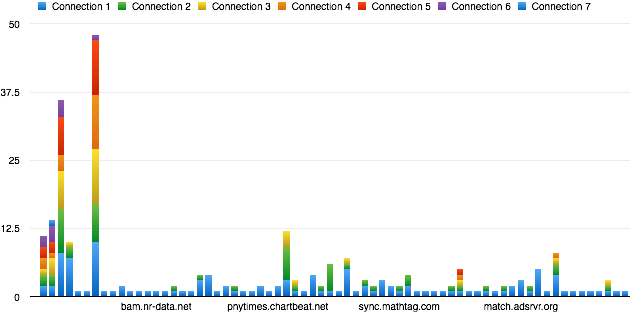
\includegraphics[scale=0.8]{Charts/objectchart1.png}
}
}
}
\vspace*{-0.6cm}
\begin{center}Figure 2: No. of objects downloaded on each TCP connection per domain - Vox (only some domain names are shown)\end{center}

%%%%%%%%%

{\bfseries Q4e. Improving Running Time: }
\\ Some points of improvement are as follows:
\begin{itemize}
\item \textbf{Managing Data Distribution:} In the implemented downloader, objects belonging to the same domain are distributed to different threads, taking into consideration the maximum objects a connection can handle at any given time. A better way to carry out this distribution would be to ensure every TCP connection gets (more or less) an even split in terms of the size of data being downloaded on the same, to ensure maximum benefit of parallelization. The file sizes can be taken from the HAR file. As for the HTTP/HTML standards, incase each reference comes with the content size, this strategy can be implemented for a browser, i.e, if a html page contains an image, if it saves the size of the image along with the location, the aforementioned strategy can be implemented.
\item \textbf{Scheduling of Threads:} In the implemented version of the downloader, for a given domain, at most $K$ ($K$ $=$ \texttt{(TCP connections)$_{max}$}) threads are spawned, each establishing its own TCP connection. Then, the downloader waits for all the threads to join, before continuing, in order to ensure that at most $K$ connections are opened at any given time to the server. This can be improved by not waiting for the thread join. Instead, at the end of each thread execution, another thread can be spawned then to handle the next batch of requests. This can be used, in conjunction with the aforementioned improvement to ensure the newly spawned thread takes up an optimal number of objects instead of the maximum allowed number of objects, so as to, again, maximize the benefits of parallelization.  
\item \textbf{Number of TCP connections opened to a domain:} The HAR file can be used to infer the maximum number of TCP connections that a server allows in parallel(i.e if the server places a cap on the maximum allowed connections). Using this information, we can dynamically allocate the value of $K$ for different domains for the case of large files; so that the overhead of creating new threads and making a new TCP connection does not outweigh the benefit of parallization. 
\item \textbf{Congestion Sensitivity:} Since the network conditions matter a lot for page load times, it only makes sense to exploit the congestion data if possible. A simple way to do this would be to measure the RTT of each connection and then allocate objects for download depending on the RTT. Hence, if one of our sockets uses a path with higher congestion, we would download less data on it.
\item \textbf{Fractional Requests:} In the case that the server sets a cap on the bandwidth allocated to a single TCP connection, large objects can be requested in chunks on separate TCP connections, with each TCP connection requesting for a fraction of the file.
\end{itemize}

\end{document}